\graphicspath{ {img/RSM/} }
\chapter[Response Surface Methodology for Efficient Spectrum Reuse in Cellular Networks][RSM for Efficient Spectrum Reuse in Cellular Networks]{Response Surface Methodology for Efficient Spectrum Reuse in Cellular Networks}
\section{Introduction}\label{RSM_sec_intro}
Approximately every decade, a new cellular access technology is developed and introduced in the market.
However, because not all users upgrade their terminals at the same pace, the operators have to keep their legacy networks working, and the spectrum assigned to these old networks becomes gradually more and more underused. 

One way to increase the spectrum efficiency is to allow the users of the newest networks to opportunistically access the spectrum of the legacy networks. Applying the concepts of cognitive radio \cite{ref:Goldsmith2}, the terminals of the newest network would be the secondary users (SUs), and the terminals of the legacy network would be the primary users (PUs). The secondary access to the spectrum of the primary (legacy) network should not cause noticeable degradation to PU transmissions. 
In this scenario, the operator owns and control both the primary and the secondary networks, and therefore can establish the rules for secondary access and monitor the impact of these rules on the performance of both SU and PU transmissions.
However, we assume \textit{no modifications on the legacy network}, implying that the operation of the secondary network is \textit{transparent} to the primary network.
%The operator could establish the rules for secondary access but we assume no signaling between the primary network and the SUs.

We consider that the SUs establish point-to-point connections among them (cognitive pairs) in an ad-hoc fashion. 
%This ad-hoc network enables multiple applications such as relying devices to increase 4G indoor coverage, device-to-device communications, or increasing the bandwidth of a small cell providing offloading services. 
%Typically, secondary spectrum access is based on occupying either temporal or spatial spectrum holes (opportunities). 
We propose a semi-decentralized secondary access scheme allowing each SU to access a set of primary frequency bands using either temporal or spatial spectrum holes (opportunities). By giving more access options to each SU, this approach can outperform previous, more limited, mechanisms. 
To fully exploit its potential, we describe an on-line algorithm that, with very small computational and signaling overhead, allows the system to learn the optimal SU access policy in terms of capacity.

%consists on exploiting both strategies simultaneously, combining them into an hybrid access scheme.

\subsection{Related Work and Contribution}

Other works have proposed the combination of temporal and spatial sensing by the SUs \cite{ref:Hybrid}, \cite{ref:Hybrid2}, \cite{ref:HybridVehicular}, \cite{ref:Hybrid3}. Works like \cite{ref:Hybrid} and \cite{ref:Hybrid2} consider a single secondary transmitter and exploit information from spatial sensing to improve the performance of temporal sensing. The single transmitter model is also applied in \cite{ref:HybridVehicular} for vehicular networks.
In \cite{ref:Hybrid3} the capacity is optimized by randomizing the access strategies, but for a single PU, single SU scenario.
However, the motivational scenario of our work comprises multiple secondary transmitters with multiple primary base stations. Thus, we must consider relevant features that are not captured by the single transmitter model, such as the inter SU-interference and the frequency reuse in a cellular structure.

In cellular networks, previous works as \cite{ref:Cellular} and \cite{ref:Cellular2} have addressed spatial spectrum reuse by a secondary network. However, these works assume that the secondary users only scan one frequency. As pointed out by their authors, scanning all the frequencies would improve the performance. 
In contrast, we follow this latter approach, mixing it with the exploitation of temporal opportunities. 

Our contribution in this work is a semi-distributed mechanism for opportunistic spectrum access combining access over temporal and spatial opportunities, in which \textit{all the spectrum of the system can be made available} to each SU. An improvement with respect to previous works is that our method is especially conceived for cellular networks, considering multiple PU transmitters within a cell structure. The system is evaluated in a realistic setting considering irregular cell shapes. And, the most important feature, \textit{the system is capable of learning the optimal probability distribution over the frequency bands of the cellular network}.
The learning algorithm applies the response surface methodology (RSM) \cite{ref:RSM_book}, which is a novel and promising approach to address interference management problems.

%We also introduce the new concept of \textit{dual tessellation}, which characterizes the spatial opportunities in cellular scenarios with frequency reuse.

In the following section we describe the system. Section \ref{sec:Formulation} formulates the design problem and Section \ref{sec:RSM} presents the RSM algorithm to solve it. Finally, Sections \ref{RSM_sec_results} and \ref{RSM_sec_conclusion} presents the numerical results and the conclusions of this work.

\section{System description}\label{RSM_sec_modell}
The system considered comprises: a legacy cellular network (primary network), a secondary network establishing ad-hoc point-to-point links, and a secondary access controller (SAC) which monitors the system performance and broadcasts the operation parameters of the SU access strategy (with small signaling overhead, as we discuss in Section \ref{sec:RSM}).
The primary network contains base stations (PBSs) and primary users (PUs).
Each PBS covers a certain geographical area (primary cell) and is assigned a frequency band different from its adjacent cells.
%Dividing all the covered region into cells (tessellation) increases the capacity of the wireless access network.
We assume a frequency reuse scheme of 7 frequency bands (reuse factor 7), denoted by $f_{1},\ldots,f_7$. Nevertheless, the proposed method can be applied to other reuse factors as well.
Each frequency band is divided into $2N$ orthogonal channels ($N$ downlink and $N$ uplink channels).
Secondary access is constrained to downlink channels.
Time is divided into equal duration time-slots, which is usual in most cellular systems.
%Time is divided into time-slots and 
The data transmitted over a single PU channel in a time-slot is referred to as \textit{packet}.

The secondary network consists of pairs of secondary users (SUs) entering and leaving the system in an ad-hoc fashion. 
This network model can characterize femtocells, terminals acting as relays, or any short-range transmission using available spectral resources of the legacy cellular network. 
%The benefit to the SUs can be improving its capacity, coverage or interference management. 
The SAC is associated to the network to which the SUs belong. 
In particular, we assume that the SUs are the users of a new generation cellular network. 
Because both networks (the new generation network and the legacy one) belong to the same operator, we consider that the SAC can retrieve some information from the legacy network.  

The SUs can detect the power of the pilot tones of the neighboring PBSs. With this information (and possibly with the aid of the SAC) each SU can infer its position with respect to the surrounding cells and therefore be aware of the PBS power levels from each frequency band. Indeed, the SU does not need to estimate exactly these PBS power levels, it just needs to establish an ordering of the frequencies $f_1,\ldots,f_7$ from lower to higher PBS power level.
For a generic SU, let $\phi = (\phi_1,\ldots,\phi_7)$ be the vector of frequencies ordered in increasing received power, %i.e. $P_{\phi_1}<\ldots<P_{\phi_7}$, where $P_{\phi_i}$ denotes the PBS power in band $\phi_i$.
which clearly depends on the location of the SU.
%, its associated $\phi$ vector is a specific permutation of the frequency set $\left\{f_1,\ldots,f_7\right\}$. 
Note that $\phi_7$ corresponds, in general, to the frequency band of the primary cell where the SU is located.

\textbf{Example}. In Figure \ref{fig:scheme}, any SU located in area A has $\phi_1 = f_1$ (similarly, any SU in area B has $\phi_1 = f_2$). But because each SU is closer to a different PBS, $\phi_7 = f_5$ for SU 1, and $\phi_7 = f_6$ for SU 2. These SUs have also different values of $\phi_2$ and $\phi_4$.

\begin{figure}[!t]
\centering
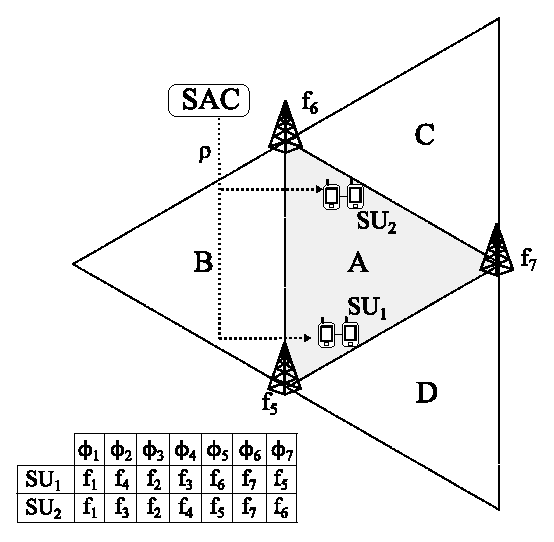
\includegraphics[scale=0.75]{scheme.eps}
\caption[]{Example of the system with 2 SU pairs. Every SU in area A associates $f_1$ to $\phi_1$. The remaining $f_j$-$\phi_i$ associations for each SU depend on how close the SU is to areas B, C or D. The SAC broadcasts a vector of operation parameters $\rho$ to the SUs.}\label{fig:scheme}
\end{figure}

%\textbf{Example.} Let us consider a primary network using an hexagonal cell structure with reuse factor 7. Se considera que R = 5. Se accede a $f_{1^{st} choice}$, $f_{2^{nd} choice}$, $f_{3^{rd} choice}$, $f_{4^{th} choice}$ mediante spatial access y a $f_{5^{th} choice}$ mediante temporal access.

%En la figura \ref{fig:scheme} se puede ver la frecuencia $f_{1^{st} choice}$ asociada a cada �rea. As�, el usuario secundario SU$_{1}$ tendr� como $f_{1^{st} choice}$ = $f_1$, ya que es la frecuencia que llega con menor potencia al �rea en que se encuentra. Como $f_{2^{nd} choice}$ se toma la $f_{1^{st} choice}$ de la secci�n de �rea m�s cercana a la que se encuentra SU$_1$ que es D. Por tanto $f_{2^{nd} choice}$ =  $f_4$ y as� sucesivamente. Por �ltimo se puede observar como la frecuencia  $f_{5^{th} choice}$ corresponde a la de la estaci�n base m�s cercana, es decir, a la de la celda primaria donde el SU se encuentra. Al estar tan cerca de la estaci�n primaria, el SU puede obtener informaci�n de qu� canales est�n ocupados y acceder a los libres (temporal access).


%Un SU cualquiera, dependiendo de su ubicacion, recibe unas frecuencias con mayor intensidad que otras. Es decir, hay una frecuencia que recibe con una potencia menor que todas las demás que llamaremos $f_{1^{st} choice}$. La frecuencia que recibe con la segunda menor potencia la denotamos con $f_{2^{nd} choice}$ y así sucesivamente hasta $f_{7^{th} choice}$ que es la frecuencia que se recibe con mayor potencia y, por tanto, corresponde a la celda primaria en la que se encuentra el SU. Obviamente, la frecuencia $f_i$ asociada asociada a cualquier frecuencia $f_{j^{th} choice}$ varía con la ubicacion del SU.
%El hecho de que un SU no reciba potencia de alguna de las estaciones también aporta informacion de la ubicacion del mismo

When an SU transmits over any band $\phi_i$, it may cause some interference to the PUs of the closest cells using this band (and the same channel within this band). In general, the level of SU interference caused at PU receivers is proportional to the ordering index $i$ of the selected band $\phi_i$, i.e. a single SU transmission over $\phi_1$ causes generally less interference than an SU transmission over $\phi_2$, and so on.
%The channels in $\phi_1$ can therefore be considered as \textit{spatial opportunities}, \cite{ref:DualTesselation}.
%Multiple previous works consider that secondary access occurs only in \textit{spatial opportunities}, which in our case corresponds to restrict the access of each SU to $\phi_1$ in its $\phi$ vector.
In our system, the classic strategy of occupying exclusively \textit{spatial opportunities}, implies that each SU only tries to access over $\phi_1$.
However, what really matters is the aggregate interference at the receivers.
Note that, in accordance to the ad-hoc nature of the secondary network (small SU transmission range, low antenna heights, indoor locations sometimes) the SINR at the PU receivers can still be acceptable even if the interference from some SUs is a bit higher, i.e. if some SUs select other bands different from $\phi_1$. 
The potential benefit of giving more frequency band options to the SUs is to decrease the inter-SU interference, increasing the capacity of the secondary network.

%Sin embargo lo que importa es la interferencia agregada en los receptores. Dado que la red SU es ad-hoc, con poca potencia, repartir las transmisiones por distintos phi puede conllevar interferencia tolerable en los PUs y mucha menor interferencia inter-SU.
%Because of its ad-hoc nature, the power of an SU transmission on each channel can be very small compared to a PBS transmission.
%%we should take into account that the transmission power of a SU terminal on each channel can be very small compared to a PBS. 
%More importantly, while the typical location of a PBS (outdoors and on top of a relatively high building) is intended to provide coverage to a wide area, a secondary transmitter is usually a user terminal, and its location (indoors or outdoors at small heights) will cause the SU signal power to decrease faster with distance compared to the transmission of a PBS.
%Therefore, in a system with high secondary activity, it is the aggregated interference at the PU receivers what should be kept under a desired level. 

Besides, when an SU tries to access the band of a close PBS, i.e. a band associated to a higher interference power such as $\phi_7$, the SU can perform \textit{PU activity detection} on the channels within the band \cite{ref:Goldsmith2}. This activity detection allows the SU to detect free channels before starting transmission, and to stop SU transmission when detecting overlap with PU transmissions. The closer the SU is to the PBS, the more reliable is the PU activity detection and therefore the less impact on PU communication.
The free channels in $\phi_7$ are identified as \textit{temporal opportunities} \cite{ref:DualTesselation} in previous works.
%por tanto no est� claro que es mejor si acceder a phi 1 o a phi 7.
%Regarding the SU interference at the PU receivers, the following considerations should be highlighted.
%Because of its ad-hoc nature, the power of an SU transmission on each channel can be very small compared to a PBS transmission.
%%we should take into account that the transmission power of a SU terminal on each channel can be very small compared to a PBS. 
%More importantly, while the typical location of a PBS (outdoors and on top of a relatively high building) is intended to provide coverage to a wide area, a secondary transmitter is usually a user terminal, and its location (indoors or outdoors at small heights) will cause the SU signal power to decrease faster with distance compared to the transmission of a PBS.
%Therefore, in a system with high secondary activity, it is the aggregated interference at the PU receivers what should be kept under a desired level. 
%When SUs exploit temporal or spatial opportunities, they are in fact adopting the primary or the dual tessellation respectively. 
%However, the capacity of each cell (primary or dual) is limited for secondary users as well, because of the intra and inter cell interference, and the limitation in the number of available channels when using temporal opportunities.
%One way to increase the capacity for the secondary network is to simultaneously use the primary and the dual tessellation, therefore duplicating the area where each frequency band can be used by the secondary terminals. This approach is the \textbf{hybrid access} and comprises the following 3 steps:

As we showed in \cite{ref:DualTesselation} the typical strategies of using only spatial opportunities ($\phi_1$ channels) or only temporal ones ($\phi_7$ free channels) are not optimal, and an hybrid scheme combining both types of access increases the capacity of the system.
%In our previous work \cite{ref:DualTesselation} we showed that an \textit{hybrid access} combining spatial opportunities ($\phi_1$ channels) with temporal opportunities ($\phi_7$ free channels) increases notably the capacity of the secondary access network, and is compatible to keeping the SU interference at PU receivers below the desired levels.
The challenge was to find the optimal balance between the fraction of the SU population exploiting each type of spectrum opportunities. %exploiting temporal opportunities and the SUs using spatial opportunities.
In this work we incorporate a learning strategy to address this issue, and extend the hybrid access idea allowing the SU to use 3 or more bands from its $\phi$ vector.%, and incorporate a crucial learning feature.

Let $R$ be the number of bands that an SU can use. We define the $R$-dimensional vector $\mathbf{\rho}=(\rho_1,\ldots,\rho_R)$, where $\rho_i$ denotes the probability of using band $\phi_i$, except for $\rho_R$ which always corresponds to the probability of using band $\phi_7$ (pure temporal access). Therefore, $0\leq\rho_i\leq 1$ for $i=1,\ldots,R$, and $\sum_{i=1}^{R} \rho_i = 1$. Let $\mathcal{P}$ denote the set of $R$-dimensional vectors fulfilling these conditions.

The following steps summarize the \textbf{system operation}:
\begin{enumerate}
	\item The SAC periodically updates the vector $\mathbf{\rho}$ and sends it to the SUs.\footnote{It is advisable to divide the system into relatively homogeneous regions in terms of PBS density, traffic intensity and type of terrain, so that a suitable $\rho$ can be found for each region.}
%. Each region should be homogeneous in terms of propagation conditions, PBS deployment pattern, and traffic intensity, so that the same $\rho$.}
	\item Each SU builds its own $\phi$ vector by scanning the PBS pilot tones on each frequency band. This vector only needs to be updated when the SU changes its location. 
	\item Before transmitting, an SU randomly selects one band, $\phi_i$ from its $\phi$ vector, according to the probability distribution $\mathbf{\rho}$, i.e. $P(\text{select band }\phi_i)=\rho_i$.
	\item If the SU is capable of detecting enough PBS power in $\phi_i$ to perform PU activity detection, then the SU tries to access over temporal opportunities, occupying only channels free of PU activity. Otherwise, the SU will access any channel with a sufficiently low SINR (considering also the interference from other SUs).% to occupy some channels of the primary cell where the secondary transmitter is in.
	\item Periodically, the SAC retrieves information from both the primary and the secondary networks, particularly performance measures, which are taken into account to update vector $\mathbf{\rho}$.
\end{enumerate}
This mechanism allows a quasi-decentralized resource allocation. The SAC only needs to \textit{announce} the vector $\mathbf{\rho}$ and retrieve small pieces of information measured at the terminals. The signaling overhead is therefore very low, especially compared to a centralized channel allocation by the SAC. If $\mathbf{\rho}$ is properly adjusted, the SUs will allocate themselves over the legacy spectrum, autonomously, efficiently, and with a low impact on the primary network.
Moreover, $\mathbf{\rho}$ can be learned by the SAC with the RSM scheme explained in Section \ref{sec:RSM}.

Note that the interference from the SUs using $\phi_7$ or $\phi_6$ may be very intense but, thanks to the PU activity detection in closer cells, it should be infrequent and last short periods of time (depending on the detection accuracy).
On the other hand, the interference from the SUs using bands that usually do not allow PU activity detection (e.g. $\phi_1$ or $\phi_2$) will be sustained over time, but will be less intense (similar to the co-channel interference from other PBSs).
To properly adjust the vector $\mathbf{\rho}$ we should combine the effects of these two types of interference into a single performance metric for the PUs: the probability of correct packet reception per time-slot.
For the SUs, the metric of interest is the achieved capacity. Next section formalizes the problem in these terms. 

\section{Problem Formulation}\label{sec:Formulation}
In this subsection we define the performance metrics for both the PUs and SUs and formulate the problem that the SAC needs to solve to determine the $\rho$ vector.
%In this section we define the performance metrics and formulate the problem that the operator needs to solve to determine the $\rho$ vector.

Let us consider a secondary network with a given traffic intensity characterized by its arrival rate per area unit, and a random transmission time.
As stated above, the vector $\rho$ determines how the SUs distribute themselves over the available spectrum and the proportion of SUs using PU activity detection. In consequence, the SINR at each PU or SU receiver depends on $\rho$.
%Time slots are numbered by $t=1,2,\ldots$.
Let $N_{t}^{SU}$ and $N_{t}^{PU}$ denote the number of SUs and PUs in the system, respectively, at time-slot $t=1,2,\ldots$.
The SINR over time at an SU receiver $s\in\left\{1\ldots N_{t}^{SU}\right\}$, is a discrete time stochastic process induced by $\rho$, and denoted by $\Gamma_{t}^{s}(\rho)$. 
%Similarly $\Gamma_{t}^{PU}(\rho)$ refers to the SINR process at a PU.
The expected normalized capacity per active SU pair is given by
\begin{equation}\label{capacityfunc}
C_{s}(\rho) = E\left\{\underset{T\rightarrow\infty}{\text{lim}}\frac{1}{T}\sum_{t=0}^{T}\sum_{s=1}^{N_{t}^{SU}}\frac{\text{log}_{2}\left(1+\Gamma_{t}^{s}(\rho)\right)}{N_{t}^{SU}C_{\text{max}}^{S}}\right\}
\end{equation}
\noindent
where $C_{\text{max}}^{S}$ is the maximum achievable SU capacity per Hertz. The expectation is taken over $\Gamma_{t}^{s}$ and $N_{t}^{SU}$.\footnote{Note that the traffic intensity in a cellular communication network varies during a day, but if it is observed during a smaller time window, e.g. 1 hour, the traffic arrival process can be considered stationary, with constant intensity.}
At a PU receiver, it is assumed that a data packet transmitted on time-slot $t$ is correctly decoded if its SINR, $\Gamma_{t}^{PU}$, is greater than a given detection threshold, $\gamma^{PU}$. Then, the probability of correct detection at a PU is defined as 
\begin{equation}
P_{c}(\rho) = E\left\{\underset{T\rightarrow\infty}{\text{lim}}\frac{1}{T}\sum_{t=0}^{T}\sum_{j=1}^{N_{t}^{PU}}\frac{\mathbb{I}_{\left\{\Gamma_{t}^{j}(\rho)>\gamma^{PU}\right\}}}{N_{t}^{PU}}\right\}
\end{equation}
%$P_{c}(\rho) = P\left(\Gamma_{t}^{PU}(\rho)>\gamma\right)$.
\noindent
where $\Gamma_{t}^{j}$ refers to the SINR process at the $j$-th active PU, and $\mathbb{I}_{\left\{z\right\}}$ is an indicator function which equals 1 if condition $z$ holds, and equals 0 otherwise.

Therefore, the objective of the SAC is to find $\rho$ solving the following problem
\begin{equation}\label{main_problem}
\begin{array}{l}
\underset{\rho}{\text{max}}\;C_{s}(\rho)\\
\text{s.t.}\\
P_{c}(\rho) \geq P_{c,\text{min}}\\
\rho\in\mathcal{P}
\end{array}
\end{equation}
where $P_{c,\text{min}}$ denotes the minimum acceptable $P_{c}$.

Finding an optimal $\rho$ is a challenging task because the (multiple) SINR stochastic processes capture the interaction of a random number of randomly located terminals with fading effects among each pair of them. 
%The traffic intensity of each network is clearly a relevant factor to consider
Moreover, these processes and the decision vector $\rho$, take values from continuous spaces, and therefore conventional dynamic programming techniques result infeasible.
%And the SAC can do that by observing realizations of the random variables $C_{s}(\rho)$ and $P_{c}(\rho)$.
%This is a \textit{stochastic optimization problem with stochastic constraints}. 
The problem (\ref{main_problem})�is, in fact, a \textit{stochastic optimization problem with stochastic constraints} \cite{ref:RSM_book}.
As usual in this type of problems, the SAC has to dynamically \textit{learn} an optimal $\rho$. 
One feasible way to address it is by means of Surface Response Methods (RSM) \cite{ref:RSM_restr}. However, the inclusion of stochastic constraints introduces high complexity in the formulation. In the following section we develop the particular case in which $P_{c,\text{min}}$ is sufficiently low for condition $P_{c}(\rho)\geq P_{c,\text{min}}$ to hold at the optimal $\rho$ (in numerical results, $P_{c}(\rho)$ at the optimal $\rho$ is never less than $5 \%$ of the $P_{c}$ obtained in absence of SU access). This allows us to remove the stochastic constraint regarding $P_c(\rho)$. We leave as future work the inclusion of constraints in the RSM formulation.

%performance del SU (formula)
%performance del PU (formula)

%problema a resolver

%version simplificada

\section{Response Surface Method (RSM) Algorithm}\label{sec:RSM}
The aim of the algorithm is the maximization of the expected value of the average capacity function (\ref{capacityfunc}) on a closed convex feasible domain $\mathcal{P}\subset\mathbb{R}^{R}$ for the input vector $\rho$, that is, to find a $\rho$ approximately solving 
%$\underset{\rho\in\mathcal{P}}{\mbox{arg max }}C_{s}(\rho)$.
%\begin{equation}
%\label{max_problem}
%\underset{\rho\in\mathcal{P}}{\mbox{ max }} E\left\{\sum_{s=1}^{N_{t}^{SU}}\text{log}_{2}\left(1+\Gamma_{t}^{s}(\rho)\right)/N_{t}^{SU}C_{\text{max}}^{S}\right\}
%\end{equation}

%\begin{equation}
%\rho^{*}=\underset{\rho\in\mathcal{P}}{\mbox{arg max }}C_{s}(\rho)
%\end{equation}
\begin{equation}
\underset{\rho\in\mathcal{P}}{\mbox{ max }}C_{s}(\rho)
\end{equation}
RSM allows us to find an approximate solution to this problem by successively estimating the gradient of the objective function and using these estimations in stochastic gradient ascent steps.
At each one of these steps, numbered by $n=1,2,\ldots$, the system generates one update of the input vector $\rho_{(n)}$ according to the following expression
%Starting from an initial guess $\rho_0$, the stochastic gradient ascent generates one update of the input vector $\rho_n$ at each step $n=1,2,\ldots$. The update operation is
\begin{equation}\label{gradascent}
\rho_{(n+1)}=\rho_{(n)} + \alpha_{(n)}\hat{\nabla}C_s(\rho_{(n)})
\end{equation}
where $\hat{\nabla}C_s$ denotes the estimation of the gradient $\nabla C_s$, and $\alpha_{(n)}$ is the step-size weighting factor. A standard condition for the selection of $\alpha_{(n)}$, assuring the convergence of $\rho_{(n)}$ \cite{ref:RSM_book}, is
$\sum_{n=1}^{\infty}\alpha_{(n)}=\infty$, $\sum_{n=1}^{\infty}\alpha_{(n)}^2<\infty$.

Let us discuss the computation of $\hat{\nabla}C_s$. Given $\rho_{(n)}$ at step $n$, we consider a subdomain $\mathcal{S}_{(n)}$ of the feasible domain $\mathcal{P}$ such that 
$\rho_{(n)} \in \mathcal{S}_{(n)} \subset \mathcal{P}$.
Note that $\rho_{(n)}$ is the point at which the estimate $\hat{\nabla}C_s$ must be computed.
Therefore, we need to estimate the objective
function $C_s(\rho_{(n)})$ on $\mathcal{S}_{(n)}$, by taking samples $y^{(i)}, i = 1, \ldots, p$, of the function. 
For this, we need a finite set of points $\rho_{(n,i)}, i = 1, \ldots, p$, generally called \textit{design points}, belonging to $\mathcal{S}_{(n)}$.
These points are chosen by the decision maker (the SAC in our case), and can be, for example, random perturbations of $\rho_{(n)}$, falling within $\mathcal{S}_{(n)}$.

Let $t_{(n)}$ denote the time-slot in which the update $\rho_{(n)}$ is obtained. Given the set of $p$ decision points, the SAC can obtain samples $y^{(i)}$ by this simple procedure:
\begin{enumerate}
	\item Determine $p$ sampling instants $t_{(n,i)}=t_{(n)}+iT$ for $i=1\ldots p$, where $T$ is a sufficiently long time period for measuring performance at the SUs.
	\item At $t_{(n,i-1)}$ (where $t_{(n,0)}=t_{(n)}$), the SAC signals the design point $\rho_{(n,i)}$ to the SUs, for $i=1\ldots p$.
	\item At $t_{(n,i)}$, the SAC obtains the capacity samples from each active SU and averages them to obtain $y^{(i)}$. 
\end{enumerate}
Thus, the estimates can be expressed as
\begin{equation}
\label{simple_estimator}
y^{(i)}=\frac{1}{T}\displaystyle\sum_{k=t_{(n,i-1)}}^{t_{(n,i)}}\displaystyle\sum_{s=1}^{N^{SU}_{k}}\frac{\text{log}_{2}\left(1+\Gamma_{k}^{s}(\rho_{(n,i)})\right)}{N_{k}^{SU}C_{\text{max}}^{S}} \hspace{1em} i = 1,2,\ldots,p,
\end{equation}
%\noindent
%IDEA IMPORTANTE, PARA ASEGURAR INDEPENDENCIA ENTRE MUESTRAS Y TENER UNA CONVERGENCIA M�S R�PIDA SE PODR�A DIVIDIR EL ESPACIO DONDE SE ENCUENTRAN LOS SUS EN CONJUNTOS SEPARADOS LO SUFICIENTE PARA PODER SER CONSIDERADOS INDEPENDIENTES
%where ${\omega}^{(1)},{\omega}^{(2)},\ldots,{\omega}^{(p)}$ are independent realizations of the random element $\omega$.
%\noindent where $\mathcal{N}_{t^{(i)}}=\left\{1 \ldots N_{t^{(i)}}^{SU}\right\}$.

%Note that we are taking the samples $y^{(i)}$ over time. This implies some degree of correlation between them. 
Note that the stochastic ascent algorithm needs $p$ periods of length $T$ to upgrade $\rho_{(n+1)}$.
%An alternative approach, in which we are working as a future improvement of our proposal, is to make use of \textit{space samples}, instead of time samples, exploiting the fact that the system is large in terms of area and users. Consider, for example, selecting $p$ sets of SUs sufficiently far from each other, and associating one sample $y^{(i)}$ to each set. This way, the correlation between samples would be notably reduced and the algorithm convergence rate could be up to $p$ times faster.

The objective function $C_s$ is then approximated on $S_{(n)}$ by a polynomial response surface model $\hat{C}_s(\rho) = \hat{C}_s(\rho|\beta_0,\beta_1\ldots\beta_R)$. The coefficients $\beta_j$, are determined by least squares estimation. Therefore, the RSM-gradient estimator $\hat{\nabla}C_s(\rho_{(n)})$ at $\rho_{(n)}$ is defined by the gradient (with respect to $\rho$)

\begin{equation}
\label{gradient_estimator}
\hat{\nabla}C_s(\rho_{(n)})= \nabla \hat{C}_s(\rho_{(n)}).
\end{equation}

Thus, $C_s$ is estimated on $S_{(n)}$ by the linear empirical model

\begin{equation}
\label{linear_model}
\hat{C}_s(\rho_{n}) = {\beta}_0 + {\beta}^{T}_{I}(\rho - \rho_{n})
\end{equation}

\noindent
where
\begin{equation}
\label{linear_model_two}
{\beta}^{T} = ({\beta}_0, {\beta}^{T}_{I}) = ({\beta}_0, {\beta}_1, \ldots,{\beta}_R)^T
\end{equation}

\noindent
is the $(R+1)$-vector of unknown coefficients of the linear model. Having samples $y^{(i)}$ of the function values $C_s(\rho_{(n,i)})$ at the design points $\rho_{(n,i)}, i = 1,\ldots,p$, in $S_{(n)}$, we can obtain, by least squares, the following estimate $\hat{\beta}$ of $\beta$:

\begin{equation}
\label{LSQ_equation}
\hat{\beta} = (W^T W)^{-1} W^T y.
\end{equation}

Here, the $p\times(R+1)$ matrix $W$ and the $p$ dimensional vector $y$ are defined by

\begin{equation}
\label{matrices}
W = \left( \begin{array}{cc}
1 & \delta^{(1)} \\
1 & \delta^{(2)} \\
\vdots  & \vdots \\
1 & \delta^{(p)} \end{array} \right), \hspace{1em}
y = \left( \begin{array}{c}
y^{(1)} \\
y^{(2)} \\
\vdots \\
y^{(p)} \end{array} \right)
\end{equation}

\noindent
with $\delta^{(i)} = \rho_{(n,i)} - \rho_{(n)}$, for $i = 1,2,\ldots,p$. Note that $(W^T W)$ in (\ref{LSQ_equation}) is invertible whenever the columns of $W$ are linearly independent, which can be easily guaranteed by a proper selection of the design points. 

In case $C_s(\rho)$ is concave on $\mathcal{P}$, the RSM algorithm will approach the global optimum following the stochastic gradient ascent iterations (\ref{gradascent}). 
For the case of 2-dimensional $\rho$ vectors, $C_s(\rho)$ was concave for the numerical simulations in \cite{ref:DualTesselation}. This property has also been observed for $R>2$ dimensions in the scenarios considered in the following Section.
%The concavity of $C_s(\rho)$ was numerically in \cite{ref:DualTesselation} , and it has been also observed for $R>2$ dimensions in the numerical experiments discussed in following Section.
%HABLAR SOBRE LA CONVEXIDAD

\section{Numerical Results}\label{RSM_sec_results}
\subsection{Evaluation Framework}

This subsection describes the Monte-Carlo methodology and the scenario used to evaluate $C_{s}$. 
The primary network uses a 7-band frequency planning, as previously stated, with irregular shaped cells having an average radius $r=700$ m. We consider pathloss and multipath fading. To compute the pathloss attenuation over distance, $A(d)$ (dB), we use the following piecewise dual-slope model \cite{ref:Goldsmith}:
\begin{equation}
\begin{array}{l}
A(d) = \\
\begin{cases}
K+10\gamma_{1}\text{log}_{10}\left(d/d_{0}\right)&d_{0}\leq d \leq d_{c}\\
K+10\gamma_{1}\text{log}_{10}\left(d_{c}/d\right)+10\gamma_{2}\text{log}_{10}\left(d/d_{c}\right)&d>d_{c}\\
\end{cases}
\end{array}
\end{equation}
% $\gamma_{1}$, $\gamma_{2}$, $K$ and $d_{c}$ are typically obtained via regression fit of empirical data. 
%A relevant aspect is that the critical distance $d_{c}$ for SU transmissions is notably smaller than the critical distance for PBS transmissions, because the PBSs are located at high outdoor locations while SUs are located either indoors or on the ground. 
%\noindent were $\gamma_{1}$, $\gamma_{2}$ are the pathloss exponents, $K$ is the propagation constant and $d_{c}$ is the critical distance.
The critical distance $d_{c}$ is notably smaller for SU transmission than for PBS transmissions, because the PBSs are located at high outdoor locations while SUs are, in general, located either indoors or at ground level. 
All the signals are assumed to experience Rayleigh fading.
%Modelo de propagaci�n y fading

The area used to generate random terminal locations is a $4.2\text{ Km}\times 4.8\text{ Km}$ rectangle. We focus on the downlink channels of one frequency band.
We consider an scenario in which the primary traffic intensity is low $0.16$ $\text{Erlangs}/\text{Km}^2$, so that the average occupation of the spectrum by the primary terminals is only $5\%$. In contrast, the SU traffic intensity, $27.5$ $\text{Erlangs}/\text{Km}^2$, is high in comparison. 
%, the spectrum is highly underused by the primary terminals, and
In this case, the SU capacity is mostly determined by the inter-SU interference and the RSM algorithm is essentially performing \textit{interference management} in the SU network.
We also discuss the effect of higher PU spectrum occupation and a different SU traffic intensity.
%Therefore, traffic intensities of the primary and secondary networks are $0.2$ $\text{Erlangs}/\text{Km}^2$ and $20$ $\text{Erlangs}/\text{Km}^2$ respectively.
%For each $f_{i}$ primary cell, at each time-slot a PU starts to transmit over an available channel with some probability, related to the PU traffic intensity.
According to the ad-hoc nature of the secondary network, the average SU link distance considered is 90 m. %However, because of co-channel interference among SUs, only up to 3 simultaneous SU transmissions can take place over the same channel in the same (primary or dual) cell. 
Table \ref{RSM_table_sim_params} summarizes the simulation parameters considered.

\begin{table}
\begin{tabular}{|c|l|} \hline
\textbf{Parameter} & \textbf{Assigned value}\\\hline\hline
\textbf{Primary transmitters} & \\\hline
number of downlink channels, $N$&5\\\hline
cell radius, $r$ &700 m\\\hline
average received power at PU &$-78$ dBm\\\hline
SINR detection threshold at PU,$\gamma^{PU}$ &$-17$ dB\\\hline
baseline noise at PU ($N_{0} + I_{PU}$)&$-110$ dBm\\\hline

\textbf{Secondary transmitters} & \\\hline
average SU Tx power per channel &0.5 W\\\hline
SU link distance&90 m\\\hline
probability of PU activity detection&0.9\\\hline
probability of overlap detection &0.8\\\hline

\textbf{Propagation parameters} & \\\hline
pathloss exponents, $\gamma_{1}$, $\gamma_{2}$&$2.4$, $4.2$\\\hline
propagation factor $K$ &$46.7$ dB\\\hline
critical distance for PBS transmission&$1.2r$ m\\\hline
critical distance for SU transmission&$100$ m\\\hline

\textbf{RSM parameters} & \\\hline
dimensions of $\rho$,$R$ & $1\ldots 5$\\\hline
measuring period $T$ (in time-slots) & $300$\\\hline
number of samples per step $p$ & $3(2^{R-1}+1)$\\\hline

\end{tabular}
\centering
\caption{Parameter setting of the reference scenario used in numerical evaluations}
\label{RSM_table_sim_params}
\end{table}
%\vspace{-4pt}
\subsection{Convergence and Usage of the Frequency Bands}
Let us consider the case of 3-dimensional $\rho$ vectors, $R=3$. 
In this case, the $\rho$ vector of a particular SU is $\rho=(\rho_1,\rho_2,\rho_3)$, being $\rho_3$ the probability of trying to access the band $\phi_7$ of the primary cell where the SU is in, and $\rho_1$ and $\rho_2$ the probabilities of accessing $\phi_1$ and $\phi_2$, the bands where the SU receives less PBS power. The SU can only perform PU activity detection on $\phi_7$ channels, while the channels of the other bands are considered spatial opportunities. 
Fig. \ref{fig:ev3D} shows the values of $\rho_1$ and $\rho_2$ ($\rho_3$ is simply $1-\rho_1-\rho_2$) over consecutive update steps $n=1,2,\ldots$. The initial vector is $\rho_{0}=(0, 0, 1)$. Although $\rho_{0}$ is a rather poor initial guess, we see that the RSM algorithm stabilizes after 20 iterations. The final value is $\rho = (0.29, 0.42, 0.29)$.
Fig. \ref{fig:capacity_surface} shows the estimated value of $C_s$ as a function of $\rho_1$ and $\rho_2$. Consistently with the result obtained by RSM, the maximum values of $C_s$ lie on the line $\rho_1+\rho_2=0.7$.

\begin{figure}[!h]
\centering
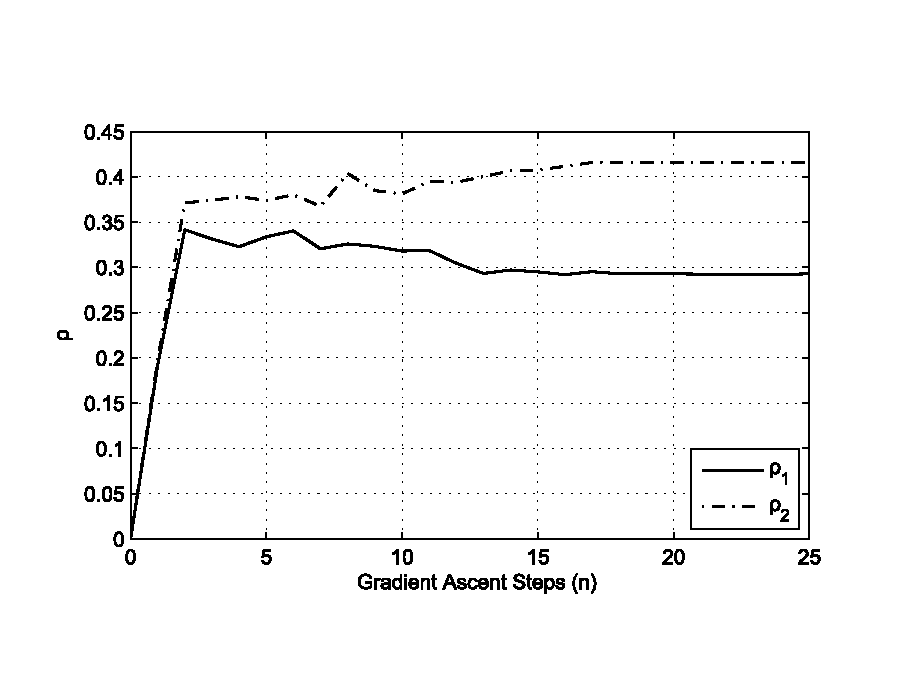
\includegraphics[scale=0.55]{evolution3D.eps}
\caption[]{Consecutive RSM updates of $\rho_1$ and $\rho_2$.}\label{fig:ev3D}
\end{figure}
%\vspace{-10pt}
\begin{figure}[!h]
\centering
\includegraphics[scale=0.55]{Barrido3Denhanced.eps}
\caption[]{Estimation of $C_s$ over $\rho_1$ and $\rho_2$.}\label{fig:capacity_surface}
\end{figure}

%\subsection{Results with $R=5$}
Let us now consider the results for $R=5$. The probability $\rho_5$ is now associated to $\phi_7$, allowing PU activity detection, while $\rho_1\ldots \rho_4$ are associated to $\phi_1 \ldots \phi_4$, where PU activity detection is assumed to be unfeasible. The initial $\rho$ vector is $(0,0,0,0,1)$. Figure \ref{fig:ev5D} shows that, in this case, the convergence of RSM is as fast as with $R=3$.
%We see that the probability assigned to each $\phi_i$, $i=1\ldots 4$, is inversely related to the PBS power received in this band.
%We see that the algorithm assigns probabilities to each $\phi_i$ in a non  
Note that, as in the case of $R=3$, the algorithm is not assigning $\rho_1$ the highest probability.
The reason is that the algorithm aims to minimize inter SU interference by separating the SU transmitters using the same band. Recall that in Fig. \ref{fig:scheme} all the SUs in triangular region A shared the same $\phi_1$ but had different values for $\phi_2$.
The aggregated probability of using spatial opportunities is $\sum_{i=1}^{4}\rho_i = 0.77$, which is higher than in the $R=3$ case.
%That is, compared to the $R=3$ case, an increased proportion of SU users are induced to select spatial opportunities. 
This result confirms the idea that, the more spectrum is available to each SU, the more spectrum the SU exploits.
Having more spectrum options per SU (higher $R$) also allows the SU network to achieve a higher capacity, as illustrated by Fig. \ref{fig:Comparativa}.
% Besides, temporal opportunities ($\phi_5$ in this case) are less used, since the PU activity 

%En este caso se puede ver como el algoritmo tambi�n converge. Es importante destacar que en este caso $\sum_i \rho_i = 0.77$. Este valor es mayor que el obtenido con $3$ dimensiones, lo cual indica que ha habido un aumento de capacidad. Esto es as� debido a que los SUs siempre prefieren oportunidades temporales antes que espaciales, debido a que reciben menos interferencias en las mismas. Cuando el tr�fico secundario aumenta mucho, las oportunidades espaciales no prov�n suficiente capacidad lo que obliga a los SUs a usar oportunidades temporales. El hecho de que la probabilidad de transmitir por oportunidad temporal sea menor implica que hay m�s capacidad en las oportunidades espaciales y esto permite a los SUs usar menos oportunidades temporales.

\begin{figure}[!t]
\centering
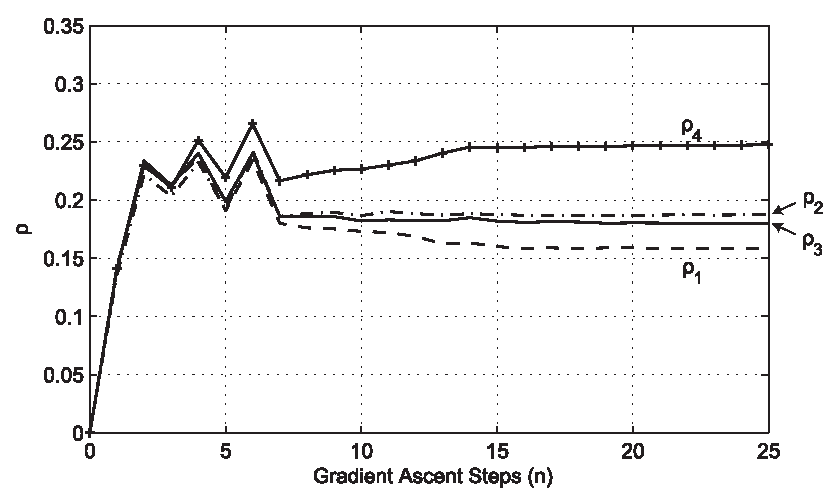
\includegraphics[scale=0.55]{evolution5D.eps}
\vspace{-10pt}
\caption[]{Consecutive RSM updates of $\rho_1 \ldots \rho_4$.}\label{fig:ev5D}
\end{figure}

\begin{figure}[!t]
\centering
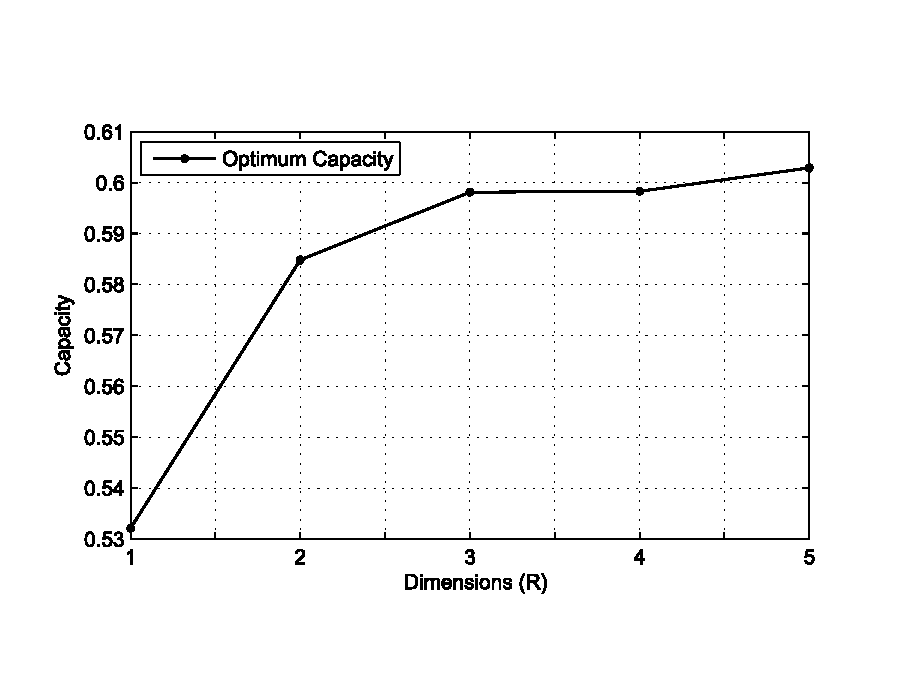
\includegraphics[scale=0.55]{comparative3.eps}
\vspace{-10pt}
\caption[]{Maximum SU capacity obtained with RSM versus the number of dimensions of $\rho$, $R$.}\label{fig:Comparativa}
\end{figure}

\subsection{Effect of the Traffic Intensity}
Fig. \ref{fig:Capacity} shows the average SU capacity attained by the RSM algorithm with $R=2$, versus the average spectrum usage by the PUs, for different SU traffic intensities. As expected, the more spectrum occupied by PU traffic, the smaller the achieved capacity. Similarly, more SU traffic implies less SU capacity. The reason of the reduction on the maximum achieved capacity is the increment of the aggregate interference power at the SU receivers, from both the PBSs and other SU pairs. 
Compared to the typical approach of exploiting only temporal opportunities, the benefit of using RSM is noticeable for every traffic situation.
In all cases, the reduction of the probability of correct detection at the PU receivers ($P_{c}$) was less than $5 \%$.
%This suggests that incorporating a tighter constraint on $P_c$, by means of RSM with stochastic constraints, would not cause a noticeable reduction on the SU capacity.
%In case the algorithm incorporated a tighter constraint on $P_c$ the SU capacity would be 

\begin{figure}[!t]
\centering
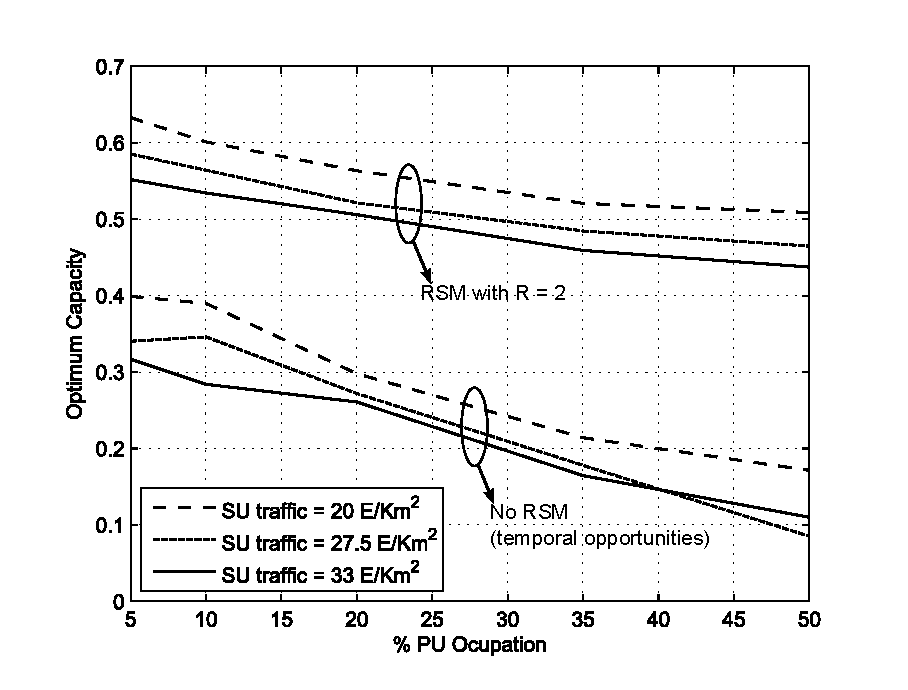
\includegraphics[scale=0.55]{optimumCapacity2Denhanced.eps}
\caption[]{Maximum SU capacity obtained with RSM under different traffic intensities. For comparision, the figure also shows the capacity for a SU network exploiting only temporal opportunities (no RSM).}\label{fig:Capacity}
\end{figure}

\section{Conclusion}\label{RSM_sec_conclusion}
Motivated by the problem of spectrum reuse in cellular networks, we presented a semi-distributed mechanism allowing the secondary network to learn the most efficient spectrum access strategy. 
This mechanism exploits both spatial and temporal opportunities, and is especially effective for interference management in highly dense secondary networks.
The learning approach is based on response surface methodology (RSM) which, according to our numerical results, improves notably the system capacity compared to usual strategies, and shows a fast convergence rate even when it is poorly initialized.
Because of that, the system can adapt its control vector $\rho$ to variations on the traffic intensity or user distribution.
Surprisingly, to the best of our knowledge, the use of RSM on this framework had not been previously reported.
Our future work is focused on incorporating performance constraints for the primary network in the RSM formulation.

%Partiendo del problema de reutilizaci�n del espectro en redes celulares, presentamos un mecanismo semi-distribuido que permite a la red secundaria aprender la estrategia m�s adecuada para acceder al espectro. El mecanismo permite explotar tanto las oportunidades espaciales como las espectrales, y est� especialmente enfocado en la gesti�n de interferencia en redes secundarias de alta densidad. La metodolog�a de aprendizaje empleada es response surface methodology. Pese a la escasa implantaci�n de RSM en este �mbito, los resultados num�ricos obtenidos muestran una notable mejor�a frente a estrategias cl�sicas en las que s�lo se explota un tipo de spectrum hole, y una alta velocidad de convergencia, incluso con inicializaciones lejanas a �ptimo. La probabilidad de recepci�n en los primarios no ha empeorado m�s del 5%, pero nuestro trabajo actual est� enfocado a a�adir restricciones de calidad en los primarios.



